\documentclass[10pt]{extarticle}
\usepackage[utf8]{inputenc}
\usepackage[labelfont=bf]{caption}
\usepackage[labelfont=bf]{subcaption}
\usepackage[width=7in,height=8.5in]{geometry}
\usepackage{fancyhdr}
\usepackage{mathtools}
\usepackage{amsmath}
\usepackage{amsfonts}
\usepackage{array}
\usepackage{booktabs}
\usepackage{listings}
\usepackage[table]{xcolor}
\usepackage[shortlabels]{enumitem}
\usepackage[mathscr]{euscript}
\usepackage{amssymb}
\usepackage{bbm}
\usepackage[hyphens]{url}

\setlength{\headheight}{24pt}
\setlength{\parindent}{0pt}

\makeatletter
\renewcommand\@biblabel[1]{#1.}
\makeatother

\pagestyle{fancy}

\rhead{Chase Austin and Jacob Wiliams \\ \today}
\chead{}
\lhead{COSC 3020 Algorithms and Data Structures \\ Assignment 03}
\rfoot{p. \thepage}
\cfoot{}

\setlength{\parindent}{0pt}
\setlength{\parskip}{4pt}
\setlength{\extrarowheight}{3pt}
\renewcommand*{\thefootnote}{\fnsymbol{footnote}}

\newcommand{\N}{\ensuremath{\mathbb{N}}}
\newcommand{\bigO}{\ensuremath{\mathcal{O}}}

\DeclarePairedDelimiter\ceil{\lceil}{\rceil}
\DeclarePairedDelimiter\floor{\lfloor}{\rfloor}

\definecolor{lightgray}{RGB}{240,240,240}
\definecolor{darkgray}{rgb}{.4,.4,.4}
\definecolor{purple}{rgb}{0.65, 0.12, 0.8}
\definecolor{green}{rgb}{0,0.8,0.1}

\lstdefinelanguage{JavaScript}{
  keywords={typeof, new, true, false, catch, function, return, null, catch, switch, 
  var, if, in, while, do, else, case, break},
  keywordstyle=\color{blue}\bfseries,
  ndkeywords={class, export, boolean, throw, implements, import, this},
  ndkeywordstyle=\color{darkgray}\bfseries,
  identifierstyle=\color{black},
  sensitive=false,
  comment=[l]{//},
  morecomment=[s]{/*}{*/},
  commentstyle=\color{green}\ttfamily,
  stringstyle=\color{red}\ttfamily,
  morestring=[b]',
  morestring=[b]"
}

\lstset{
   language=JavaScript,
   backgroundcolor=\color{lightgray},
   extendedchars=true,
   basicstyle=\footnotesize\ttfamily,
   showstringspaces=false,
   showspaces=false,
   numbers=left,
   numberstyle=\footnotesize,
   numbersep=9pt,
   tabsize=2,
   breaklines=true,
   showtabs=false,
   captionpos=b
}

\lstset{
    escapeinside={(*@}{@*)},          % if you want to add LaTeX within your code
}

\begin{document}

%%%%%%%%%%%%%%%%%%%%%%%%%%%%%%%%%%%%%%%%%%%%%%%%%%%%%%%%%%%%%%%%%%%%%%%%%%%%%%%%
\section{The memoized Held-Karp algorithm}
We prepared a memoized Held-Karp algorithm using the top-down dynamic
programming approach. This algorithm takes in an undirected, weighted complete
graph in the form of an adjacency matrix, as well as a given start vertex. It
returns the shortest tour of all vertices in the graph that begin at the start
vertex.

\subsection{The code}
\begin{lstlisting}[language=JavaScript]
///////////////////////////////////////////////////////////////////////////////
////                    The memoized Held-Karp algorithm                   ////
///////////////////////////////////////////////////////////////////////////////

// We implement a data structure for storing the visited tours. The first entry
// stores a Set of edges in the tour; the second stores the cost of the tour.
function StoreTours(edges,cost) {
  this.edges = edges;
  this.cost = cost;
}

// For comparing two Sets of edges in (sub-)tours, we implement a check to see
// whether they are the same. This was taken from code found at
//    https://stackoverflow.com/questions/31128855.
// Returns TRUE if the sets are the same, FALSE otherwise.
function sameSet(set1,set2) {
  if (set1.size !== set2.size) return false; // obvious and quick check
  for (let x of set1) if (!set2.has(x)) return false;

  return true;
}


// The Held-Karp memoized algorithm, modified from pseudocode in the lectures.
// Parameters:
//  graph => an adjacency matrix for the undirected, weighted graph.
//  unvisited => a list of unvisited vertices, defaulting to all of them
//  start => a user-specified vertex from which the tour begins
let storedTours = new Array(2);                 // Store all tours and sub-tours
  storedTours[0] = new Array();
  storedTours[1] = new Array();

function heldKarp(graph,unvisited,start) {
  // Memoization check
  for (let i = 0; i < storedTours[0].length; i++) {
    if (sameSet(unvisited,storedTours[0][i])) {
      return storedTours[1][i];
    }
  }

  if (unvisited.length <= 1) return 0;          // No tours to consider

  if (unvisited.length === 2) {
    let tour = new Set(unvisited);
    let cost = graph[unvisited[0]][unvisited[1]];

    storedTours[0].push(tour);
    storedTours[1].push(cost);
    return cost;
  } 
  
  else {
    // Filter out the start vertex
    let theRest = unvisited.filter(vert => vert !== start);

    let tour = new Set(theRest);
    let cost = Infinity;
    for (let i = 0; i < theRest.length; i++) {
      let testCost = heldKarp(graph,theRest,theRest[i]) + 
        graph[start][theRest[i]];

      if (testCost < cost) {
        cost = testCost;
      }
    }

    storedTours[0].push(tour);
    storedTours[1].push(cost);
    return cost;
  }
}
\end{lstlisting}


\subsection{Empirical time complexity}
We investigated the empirical time complexity on Chase's home computer,
running a sequence of graphs of increasing size. The results, of number
$n$ of vertices against runtime, were plotted in Excel, along with the
least-squares trendline plotted. Note that only graphs with 7--10 
vertices are plotted, because smaller graphs took less than 1 ms to run
(showing up as 0 on our timer) and the 11-vertex graph took more time than
we allotted.

\begin{figure}[ht]
    \centering
    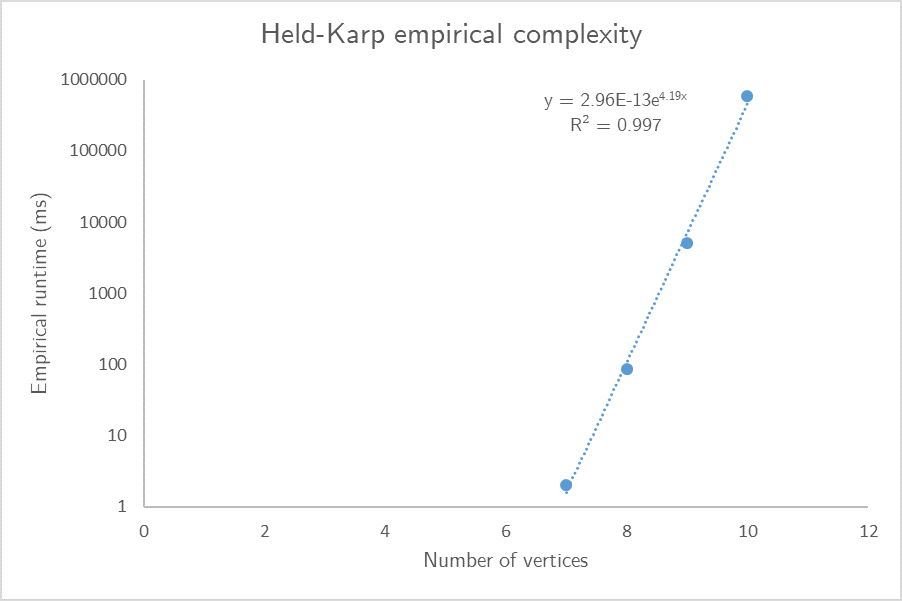
\includegraphics[width=4in]{heldKarp_trendline.png}
    \caption{The empirical runtime for the Held-Karp algorithm.}
    \label{fig:my_label}
\end{figure}

Given the empirical runtime trendline shown, we would expect a graph on 11
vertices to take approximately $(2.96 \cdot 10^{-13})e^{(4.19 \times 11)} =
30,755,612$ milliseconds, or about 8.5 hours. This is well above the one-
hour threshold.


\subsection{Worst-case asymptotic complexity}
It is well known that among a set of size $n$ there are $2^n$ total subsets.
This is also the number of tours and sub-tours of a graph with $n$ vertices.
In the worst case, the Held-Karp algorithm stores each of them in the cache;
furthermore, each one requires storing up to $n+1$ values (the $n$ vertices
visited in the tour and the cost associated with it). So the total space
complexity of the Held-Karp implementation is $\Theta(n \times 2^n) = 
\Theta(2^{n+1})$.

Because of memoization, the algorithm will spend (more than a constant amount 
of) time on each subset no more than once. Thus, in the worst case, the main
body of the algorithm will run $2^n$ times. The base case of the algorithm
(when the size of the subtour is $\leq 2$) requires only constant time to run,
but the recursive part may require time linear in the number of vertices,
so this part of the algorithm requires $\Theta(n \times 2^n) = \Theta(2^{n+1})$
time as well. The memoization check can also take $\Theta(2^n)$ time, since
there may be that many entries stored in the cache. 

Thus, the overall worst-case time complexity of this implementation of the
Held-Karp algorithm is $\Theta(2^{n+1})$. \medskip



\section{The stochastic 2-opt local search}
We also prepared a stochastic 2-opt local search algorithm. This code is not
guaranteed to produce an optimal result, but it runs much more quickly than
does the Held-Karp implementation. Like the Held-Karp algorithm, the 2-opt
stochastic local search algorithm takes an adjacency matrix for an undirected,
complete graph and a starting vertex as input and returns an approximate cost
for the shortest tour starting at the start vertex.


\subsection{The code}
\begin{lstlisting}[language=JavaScript]
///////////////////////////////////////////////////////////////////////////////
////              The 2-opt stochastic local search algorithm              ////
///////////////////////////////////////////////////////////////////////////////

// We begin with helper functions: one to randomly reverse part of a given
// tour; and one to randomly generate a tour (e.g., to start the algorithm).


// Randomize the elements of an array to find a random starting tour
// Found at https://gomakethings.com/how-to-shuffle-an-array-with-vanilla-js/
function shuffle(array) {
	let i = array.length,
	    temp, 
      random_i;

	// While there remain elements to shuffle...
	while (i !== 0) {
		//Pick a remaining element...
		random_i = Math.floor(Math.random() * i);
		i--;
		
    //And swap it with the current element.
		temp = array[i];
		array[i] = array[random_i];
		array[random_i] = temp;
	}
	return array;
}


// Reverse the part of the route between indices i and k, returning the
// new route.
function two_opt_reversed(route,i,k) {	
	
  // Temporary copy of the input route  
	let copy = route.slice();

	// Reverse the section of the reverse between i and k
	for (let x = i-1, z=k-1; x < k; x++) {	
		route[z] = copy[x];
		z--;
	}		
	return route;	
}

// Stochastic 2-opt local search algorithm running 100*|V|^2 times.
// Takes as input an adjacency matrix and a start vertex.
function twoOptIter(graph,start) {

  // Small graph corner cases
  if (graph.length <= 1) return 0;

  // Function global variables
  let tour = new Array(graph.length),
      cost = Infinity,
      maxIter = 100*graph.length*graph.length;


  // Generate the random tour (save for the start vertex)
  for (let i = 0; i < tour.length; i++) tour[i] = i;
  tour = tour.filter(vert => vert !== start);

  tour = shuffle(tour);

  // Find the initial cost of the tour
  for (let i = 0; i < tour.length - 1; i++) {
    cost += graph[tour[i]][tour[i+1]];
  }
  
  // Add the distance to the start
  cost += graph[start][tour[0]];
  
  // Randomize the route, checking for convergence
  for (let numIter = 0; numIter < maxIter; numIter++) {

    // Temporary tour cost
    let tempCost = 0;

    // Boundaries on which to reverse the route
    let i = Math.ceil(tour.length*Math.random()),
        k = Math.ceil(tour.length*Math.random());

    // Construct partially reversed tour and find its cost
    tour = two_opt_reversed(tour,Math.min(i,k),Math.max(i,k));

    for (let i = 0; i < tour.length - 1; i++) {
      tempCost += graph[tour[i]][tour[i+1]];
    }

    tempCost += graph[start][tour[0]];


    if (tempCost < cost) cost = tempCost;
  }

  return cost;
}
\end{lstlisting}


\subsection{Empirical time complexity}
We investigated the empirical time complexity on Chase's home computer,
running a sequence of graphs of increasing size. The results, of number
$n$ of vertices against runtime, were plotted in Excel.

\begin{figure}[ht]
    \centering
    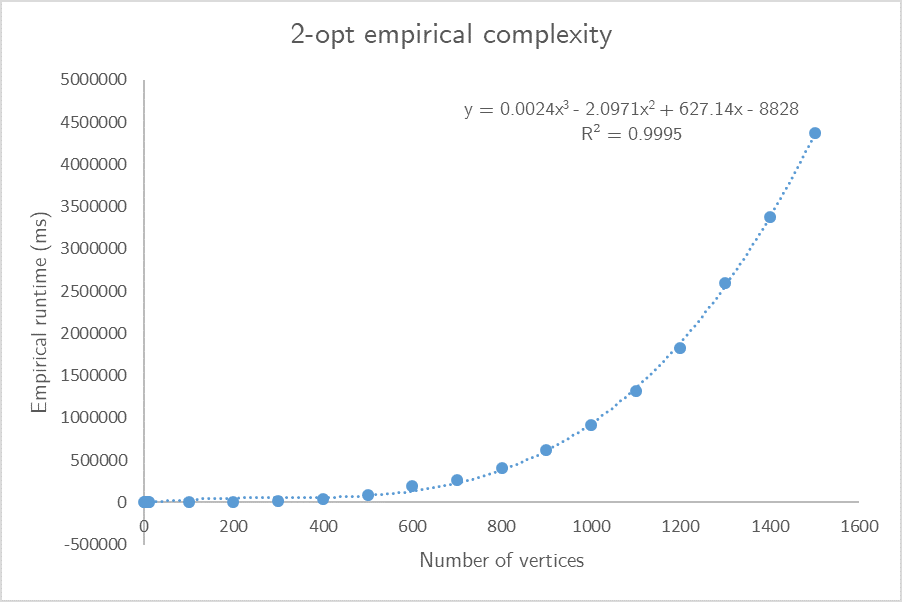
\includegraphics[width=4in]{2Opt_trendline.png}
    \caption{The empirical runtime for the 2-opt graph}
    \label{fig:my_label}
\end{figure}

The cubic curve fits the plot very well, and the longest runtime is 4,371,957 ms,
or about 1.21 hours.


\subsection{Worst-case asymptotic complexity}
First, consider the helper functions. The \verb|shuffle()| function runs in time
linear in the input size; namely, the entire initial tour, which has length $n$
for a graph on $n$ vertices. So this function runs in $\Theta(n)$ time, and 
requires only a constant amount of extra memory.

Likewise, the \verb|two_opt_reversed()| function runs in time linear in the
distance between the indices; in the worst case, it may reverse the entire 
tour array, requiring $\Theta(n)$ time. Additionally, this function creates a
temporary array, also requiring $\Theta(n)$ space in the worst case.

Finally, the main function runs exactly $100 n^2$ times, where $n$ is the 
number of vertices in the graph. We chose this number because the number of 
edges in the graph is on the order of $n^2$, so multiplying this by a moderately
large constant should give a good chance of a good approximation to the shortest
tour. The algorithm calls \verb|shuffle()| exactly once, but calls
\verb|two_opt_reversed()| once each iteration; in addition, it requires 
$\Theta(n)$ time to update the cost each iteration. Apart from the extra space
required by its helper functions, the main function requires only a constant 
amount of extra memory.

As such, the overall runtime of the stochastic 2-opt local search is
$\Theta(n + n^2 \times (n + n)) = \Theta(n^3)$, and it requires $\Theta(n)$
space. Running in polynomial time, with a fairly small exponent, and in linear
space, this algorithm is much more efficient than Held-Karp's implementation
above. \medskip



\section{Empirical comparison}
We plot the empirical runtimes for both algorithms together. Although the 10-
vertex graph finishes much more quickly on Held-Karp than the 1500-vertex
graph on the 2-opt algorithm, we predict that the 11-vertex graph will take
much longer.

\begin{figure}[ht]
    \centering
    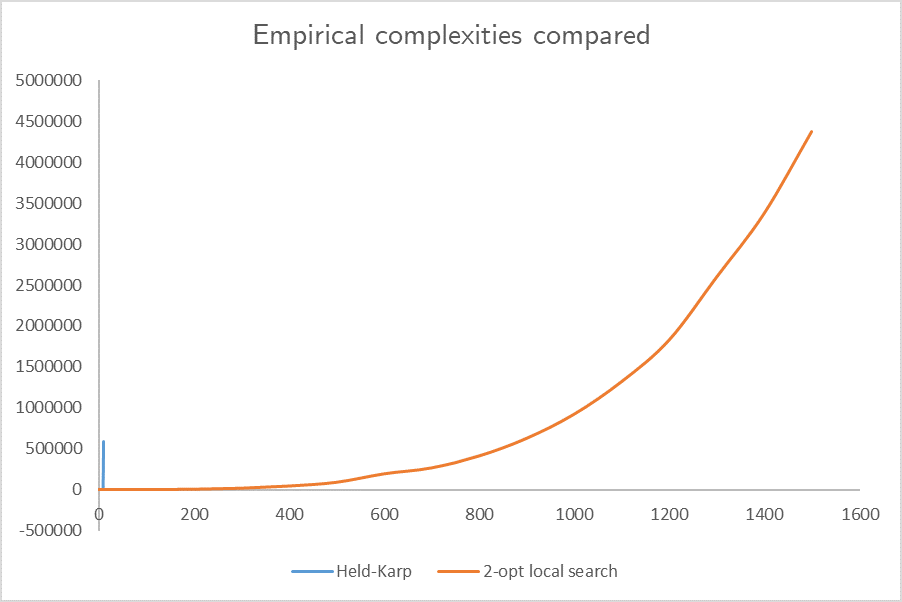
\includegraphics[width=4in]{bothGraphed.png}
    \caption{The empirical runtimes plotted together.}
    \label{fig:my_label}
\end{figure}

We also record the true shortest path (from Held-Karp) and the estimated
shortest path (from 2-opt).

\begin{table}[ht]
    \centering
    \begin{tabular}{@{}lll@{}}
        \toprule
        Number of vertices & True shortest tour & Approximate shortest tour \\
        \midrule
        0 &	0 &	0 \\
        1 &	0 &	0 \\
        2 &	6 &	6 \\
        3 &	5 &	5 \\
        4 &	14& 14 \\
        5 &	16&	16 \\
        6 &	17&	17 \\
        7 &	21&	21 \\
        8 &	19&	19 \\
        9 &	19&	20 \\
        10&	17&	19 \\
        \bottomrule
    \end{tabular}
    \caption{The shortest paths found.}
    \label{tab:1}
\end{table}

Mostly, for these small graphs, the shortest paths found are the same length.
However, the 2-opt graph finds slightly longer paths for the graphs of size
9 and 10. This is to be expected, since 2-opt stochastic local search finds
only an approximate solution to the shortest tour.


\end{document}
